\documentclass[10pt,a4paper]{article}
\usepackage[utf8]{inputenc}
\usepackage[spanish]{babel}
\usepackage{amsmath}
\usepackage{amsfonts}
\usepackage{amssymb}
\usepackage{enumitem}
\usepackage{hyperref} 
\usepackage{listings}
\usepackage{float}
\hypersetup{pdftex,colorlinks=true,allcolors=blue}
\usepackage{graphicx}
\hypersetup{
    pdftitle={PEC1},
    pdfauthor={Pablo Riutort Grande},
    pdfsubject={Identidad Digital},
    bookmarksnumbered=true,     
    bookmarksopen=true,         
    bookmarksopenlevel=1,       
    colorlinks=true,            
    pdfstartview=Fit,           
    pdfpagemode=UseOutlines,    % this is the option you were lookin for
    pdfpagelayout=TwoPageRight
}
\usepackage{listings}
\usepackage{xcolor}
\usepackage{hypcap}
\definecolor{codegreen}{rgb}{0,0.6,0}
\definecolor{codegray}{rgb}{0.5,0.5,0.5}
\definecolor{codepurple}{rgb}{0.58,0,0.82}
\definecolor{backcolour}{rgb}{0.95,0.95,0.92}
\lstdefinestyle{mystyle}{
    backgroundcolor=\color{backcolour},   
    commentstyle=\color{codegreen},
    keywordstyle=\color{magenta},
    numberstyle=\tiny\color{codegray},
    stringstyle=\color{codepurple},
    basicstyle=\ttfamily\footnotesize,
    breakatwhitespace=false,         
    breaklines=true,                 
    captionpos=b,                    
    keepspaces=true,                 
    numbers=left,                    
    numbersep=5pt,                  
    showspaces=false,                
    showstringspaces=false,
    showtabs=false,                  
    tabsize=2
}
\lstset{style=mystyle}

\usepackage{xparse}
\NewDocumentCommand{\codeword}{v}{%
\texttt{{#1}}
}
\author{Pablo Riutort Grande}
\title{Identidad Digital\\ \vspace{1cm}\textbf{PEC 2}}
\begin{document}
\maketitle
\pagebreak
\section{}
\subsection{}
La Deep Web consiste en todo el contenido de internet que no es indexado por motores de búsqueda convencionales, de tal forma, que el acceso a la Deep Web se hace difícil desde el uso cotidiano de navegadores. La mayoría de este contenido consiste en bases de datos, archivos, páginas dinámicas o páginas explícitamente restringidas a los spiders de los motores de búsqueda.\\

La Dark Net se trata de una red encriptada construida encima de la infraestructura de internet. De manera similar a los protocolos convencionales que usamos para navegar por internet, existen protocolos especiales y encriptados que utilizan internet como su infraestructura. Por tanto, acceder a esta red requiere de un software y navegadores especiales como TOR (\textit{The Onion Router}), este navegador utiliza enlaces .onion para acceder a contenido y el encaminamiento para acceder a estas páginas se hace de manera encriptada para proteger la identidad de sus usuarios.\\

La Dark Web (a menudo también referido como Dark Net y viceversa) es un subconjunto de la Deep Web y además de no ser indexado por los motores de búsqueda utiliza la Dark Net para proporcionar su contenido. La Dark Web generalmente está asociada a prácticas y otras actividades ilícitas que se aprovecha del anonimato que ofrece la Dark Net para poder ejercer estas prácticas sin ser detectadas fácilmente.
\subsection{}
Epic browser es un navegador centrado en proteger la privacidad y el anonimato de sus usuarios reduciendo la información que se puede obtener de un explorador convencional. Es un explorador cuyo modo por defecto es el de los de navegación de incógnito de otros navegadores, es decir, no guarda las cookies ni el historial de navegación y borra todos los datos almacenados en caché. Epic bloquea ads y trackers y no guarda los datos de la dirección de la página web anterior desde la cual se ha llegado a la actual (Referer header).\\
Además, las búsquedas de este explorador se hacen a través de su VPN integrada aportando así las características de privacidad de este tipo de redes.

El explorador de TOR es muy similar al de Epic en el sentido de bloquear los anuncios y trackers e incluso llegar a no permitir ejecutar código JavaScript siendo TOR otra opción muy buena para optar por la privacidad y anonimato. Ambos se centran en reducir la huella digital que pueda dejar un usuario. Sin embargo, la diferencia principal reside en que el explorador de TOR está concebido para utilizarse encima del protocol con mismo nombre. Este protocolo encripta las comunicaciones de punto a punto en la capa de transporte mientras que Epic se limita al tráfico sobre VPN.

\subsection{}
Freenet es una red P2P descentralizada y anonimizada. Funciona a través de los nodos que se conectan a la misma red, las comunicaciones entre estos nodos están encriptadas y enrutadas a través de otros nodos. Esta red funciona con usuarios voluntarios que contribuyen ofreciendo ancho de banda y una porción de disco duro para guardar archivos de la propia red. Estos archivos se mantienen vigentes en la red en función de su popularidad y son encriptados de tal forma que el usuario que los tenga físicamente no puede ver su contenido.\\
Por tanto, Freenet funciona como un dispositivo de almacenamiento masivo donde se puede acceder a un archivo mediante una clave y este contenido está distribuido a través de los nodos de Freenet.\\

TOR, al igual que Freenet, se compone de voluntarios que ofrecen sus ordenadores como nodos. La primera diferencia que encontramos en TOR respecto a una red convencional es en el encamiento y envío de paquetes que viajan entre estos nodos. El encaminamiento consiste en seleccionar 3 nodos de la red al azar y el envío conciste en encriptar en varias capas el contenido del paquete que finalmente se enviará por el camino que se constituye a través de los nodos seleccionados.\\
Cuando un usuario envía un paquete encriptado, primero lo recibe el router A del conjunto de nodos que encaminan esa conexión, este router desencripta la primera capa y envía el contenido (aún encriptado) al router B y así sucesivamente hasta que se llega al destino. Cabe destacar que los routers (u otro observador) no conocen el camino completo del paquete, sólo cuál es el siguiente nodo de la lista.
\subsection{}
En el apartado anterior se mencionaba la selección aleatoria de nodos para el encaminamiento de paquetes en la red TOR, estos nodos reciben el nombre de relays.\\
Los relays encaminan estos paquetes y ocultan el rastro que pueda dejar de tal forma que ningún observador en ningún punto del circuito pueda decir de dónde viene el paquete o a dónde va dirigido.

Los relays permiten construir circuitos de conexiones encriptadas creando así conexiones privadas en la red. Este circuito se construye de manera incremental a través de los relays. Cada relay sabe únicamente quién es su predecesor y sucesor en este circuito, de tal forma que ningún relay sabe el camino completo que un paquete debe recorrer para llegar a su destino.\\

Existen 4 tipos de relays:

\begin{enumerate}
\item \textbf{Guard relay}\\
Es el primer relay de un circuito TOR. Estos relays requieren ser estables y rápidos, tampoco permiten mandar tráfico al destino real del paquete en su política de salida.
\item \textbf{Exit relay}\\
Envía el paquete a su destino. Los servicios a los que los clientes TOR se conectan verán la IP de este relay, por tanto son los relays más críticos respecto a revelación y aspectos legales, puesto que cualquier medida legal se aplicará sobre el responsable de esta dirección IP.
\item \textbf{Middle relay}\\
Los middle relay son relays que no son de tipo guard ni exit, actúa como conexión de estos dos.
\item \textbf{Bridge}\\
Las IPs de los relays de TOR son públicas, por tanto, son bloqueables por algunos ISPs o gobiernos. Para paliar este problema, los bridges son nodos que no están listados en el directorio de TOR.
\end{enumerate}



\section{}
\subsection{}
El flujo de mensajes entre cliente y servidor para SAML sería:

magine you're the user in an environment with single sign-on and you're trying to get access to some resource on a server. The sequence of events goes like this:

You try to access the resource on the server, which in SAML terminology is a service provider. The service provider in turn checks to see if you're already authenticated within the system. If you are, you skip to step 7; if you're not, the service provider starts the authentication process.
The service provider determines the appropriate identity provider for you and redirects you to that provider — in this case, the single sign-on service.
Your browser sends an authentication request to the SSO service; the service then identifies you.
The SSO service returns an XHTML document, which includes the authentication information needed by the service provider in a SAMLResponse parameter.
The SAMLResponse parameter is passed on to the service provider.
The service provider processes this response and creates a security context for you — basically, it logs you in — and then tells you where your requested resource is.
With this information, you can now request the resource you're interested in again.
The resource is finally returned to you!

Para el flujo de comunicaciones de SAML existen 3 entidades principales de intercambio de mensajes:
\begin{itemize}
\item El Identity Provider: publica sentencias de identidad
\item El Service Provider: acepta sentencias de identidad y un perfil SSO
\item Un usuario (Principal) que intenta acceder a un recurso a través del Service Provider
\end{itemize}
El flujo de mensajes entre las 3 entidades es el siguiente:
\begin{enumerate}
\item El usuario intenta acceder a un recurso del Service Provider
\item El Service Provider comprueba si el usuario está autenticado en el sistema
\item Empieza el proceso de autenticación: El Service Provider determina el Identity Provider para el usuario y lo redirige a este.
\item El explorador envía una petición de autenticación al servicio SSO (Single Sign-On).
\item El SSO devuelve un documento XHTML que incluye la información necesario para el Service Provider en un parámetro SAMLResponse.
\item El Service provider Procesa esta petición y crea un contexto de seguridad e informa de dónde está el recurso solicitado
\item Una vez autenticado el recurso ya está disponible para el usuario.
\end{enumerate}
\subsection{}
En el caso de la práctica, el flujo de mensajes sería el siguiente:
\begin{enumerate}
\item Un usuario intenta acceder a un recurso a través del explorador
\item Spring Security ve que no es un usuario autenticado y conectará con el servidor CAS
\item El usuario se autentica en el servidor CAS y este validará los datos introducidos con los credenciales de LDAP
\item El usuario es redirigido a la web app con nuevos credenciales y permisos para acceder a diferentes secciones de las web app.
\end{enumerate}

Vemos que la similitud con el SAML es principalmente entre las entidades siendo el usuario el mismo, Spring Security el Service Provider y el CAS el Identity Provider y el flujo de mensajes algo bastante similar siendo el primer encuentro entre el usuario y el Service Provider (Spring), luego una conexión entre el Service Provider y el Identity Provider (CAS) para validar al usuario y el Identity Provider valida los credenciales de tal forma que Spring puede conceder el acceso.
\subsection{}

WebAuthn es una especificación del W3C con la participación de empresas importantes del sector tecnológico que permite a las aplicaciones web crear credenciales basados en claves públicas para la autenticación en vez de contraseñas.\\
WebAuthn se puede utilizar para el segundo factor de autenticación universal (U2F) o también para la autenticación biométrica permitiendo a las aplicaciones web utilizar credenciales específicas para ese servicio. Los atributos que se utilizan para generar estos credenciales suelen ser desconocidos para el usuario y, por tanto, se reduce el riesgo de que sean robados.\\

El sistema permite al los servidores integrarse con los servicios de autenticación de los dispositivos con funciones biométricas generando una par de claves privada y pública para la aplicación. La clave privada se guarda en el dispositivo y la pública se envía al servidor de la aplicación junto a un ID de usuario generado aleatoriamente. Una vez hecho esto, el servidor puede autenticar al usuario con la clave pública almacenada contra la privada del dispositivo. De esta forma, el servidor para a guardar una información pública del usuario como medio de autenticación.
\subsection{}
En Kerberos existen las siguientes entidades:
\begin{itemize}
\item TGS (Ticket Granting Server): Servicio de expedición de tickets
\item SPN (Service Principal Name): Nombre del recurso al que se pretende acceder
\item KDC (Key Distribution Center)
\end{itemize}
Para que un usuario pueda acceder a los recursos de una red gestionada por Kerberos deberá seguir los siguientes pasos
\begin{enumerate}
\item Un cliente solicita un ticket de autenticación al centro de distribución de claves
\item El KDC verifica los credenciales y devuelve el ticket cifrado mediante la clave secreta del TGS y una clave de sesión
\item El cliente guarda el ticket hasta que expire, en cuyo caso el gestor de sesión pedirá un ticket nuevo
\item El cliente manda el ticket al TGS con el nombre del servicio al que quiere acceder
\item El KDC verifica el ticket y que el usuario tiene permisos para acceder al recurso
\item El TGS manda una clave de sesión para el servicio al cliente
\item El servidor provee del servicio al cliente
\end{enumerate}

\section{}
\subsection{}
Recordemos que las cookies están formadas por ciertos atributos y uno de ellos es el dominio. El dominio de una cookie indica el dueño de la misa, un servidor solo puede acceder a cookies generadas por otro servidor dentro del mismo dominio. Sin embargo, cuando una cookie pertenece a un dominio diferente al de la web que se está accediendo, esta es una cookie de "terceros" (third party cookie). Generalmente, se suelen usar con fines de tracking a través de diferentes sitios web para recolectar datos del usuario que guarda esa cookie.\\

Puede afectar en la privavidad del usuario porque no se pueden gestionar desde el sitio que se está visitando, ya que al ser una cookie de otro dominio el servidor de la página que se esté visitando no tiene control sobre esta. Estas cookies van con el usuario a través distintas páginas web y recoge información constantemente de su actividad en internet.

\subsection{}

Un web beacon está diseñado para trackear la actividad de un usuario y sus actividades en una página web. Suele ser una imagen (de 1x1 píxeles) o un objeto muy pequeño que se encuentra en una página web que, cuando es visitada, guarda información variada del usuario para su posterior análisis: IP del usuario, el timestamp de la visita, la página en particular que fue visitada, etc. \\

Los web beacons también pueden encontrarse en los correos electrónicos y recoger la misma información de encontrarse en una página web como, por ejemplo, si el email fue leído, la IP que se usó para leer el email, software utilizado por el lector, etc.
\subsection{}

\subsubsection*{Periódicos y sitios de noticia}

\begin{figure}[H]
  \centering
  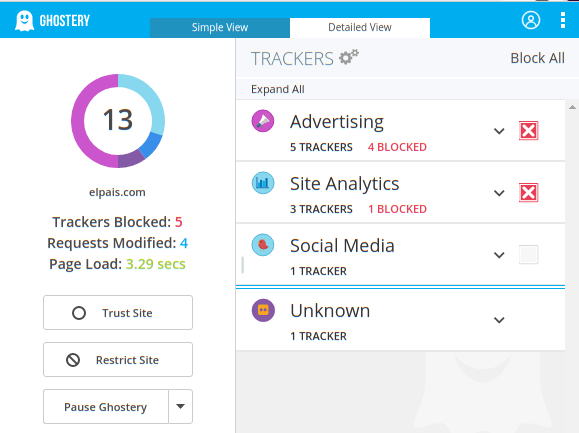
\includegraphics[scale=0.6]{ghost_elpais.png}\\
  \caption{Trackers de El País}
  \label{fig:object}
\end{figure}

\begin{figure}[H]
  \centering
  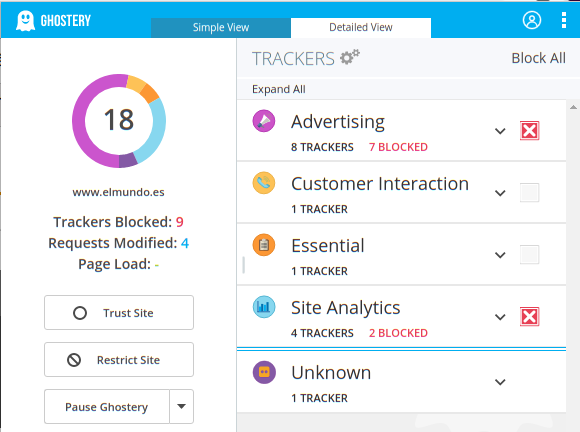
\includegraphics[scale=0.6]{ghost_elmundo.png}\\
  \caption{Trackers de El Mundo}
  \label{fig:object}
\end{figure}

\begin{figure}[H]
  \centering
  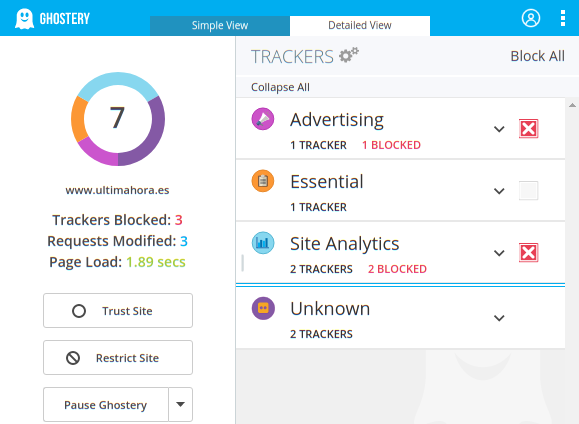
\includegraphics[scale=0.6]{ghost_ultima_hora.png}\\
  \caption{Trackers de Última Hora}
  \label{fig:object}
\end{figure}

\begin{figure}[H]
  \centering
  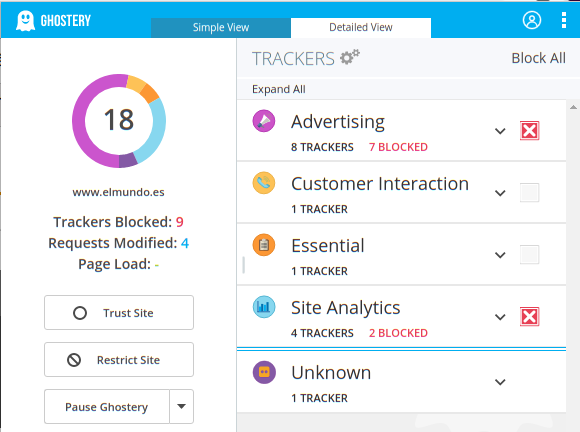
\includegraphics[scale=0.6]{ghost_elmundo.png}\\
  \caption{Trackers de El Mundo}
  \label{fig:object}
\end{figure}

\begin{figure}[H]
  \centering
  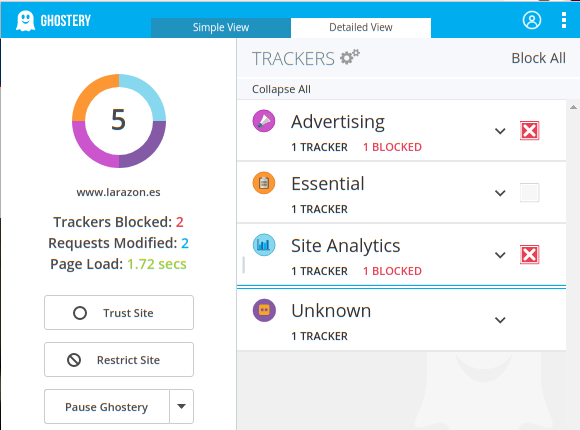
\includegraphics[scale=0.6]{ghost_razon.png}\\
  \caption{Trackers de La Razón}
  \label{fig:object}
\end{figure}

\begin{figure}[H]
  \centering
  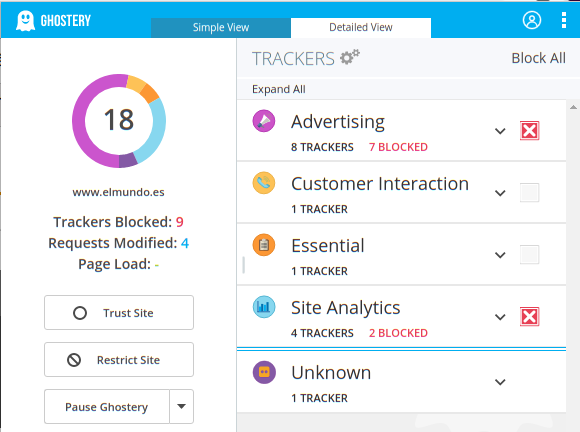
\includegraphics[scale=0.6]{ghost_elmundo.png}\\
  \caption{Trackers de El Mundo}
  \label{fig:object}
\end{figure}

\begin{figure}[H]
  \centering
  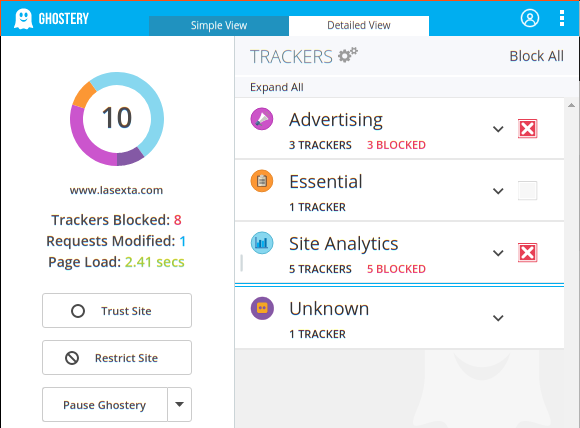
\includegraphics[scale=0.6]{ghost_la_sexta.png}\\
  \caption{Trackers de La Sexta}
  \label{fig:object}
\end{figure}

\subsubsection*{Universidades}

\begin{figure}[H]
  \centering
  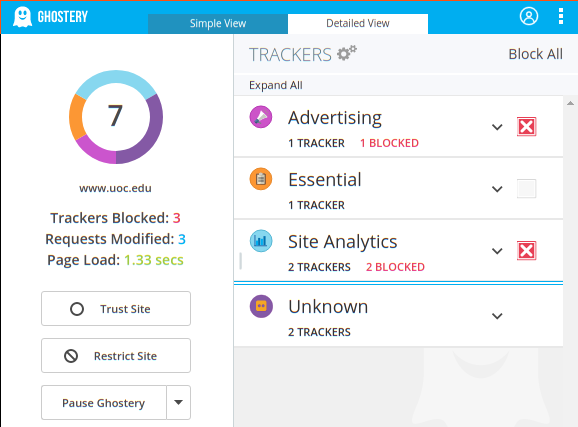
\includegraphics[scale=0.6]{ghost_uoc.png}\\
  \caption{Trackers de UOC}
  \label{fig:object}
\end{figure}

\begin{figure}[H]
  \centering
  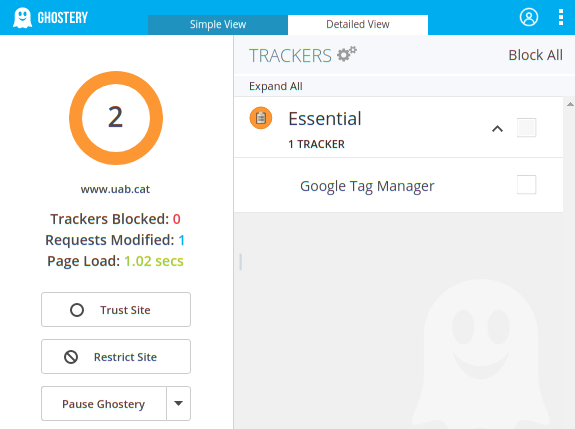
\includegraphics[scale=0.6]{ghost_uab.png}\\
  \caption{Trackers de UAB}
  \label{fig:object}
\end{figure}

\begin{figure}[H]
  \centering
  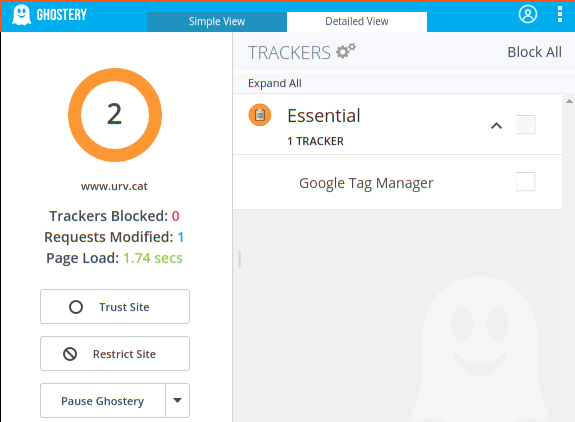
\includegraphics[scale=0.6]{ghost_urv.png}\\
  \caption{Trackers de URV}
  \label{fig:object}
\end{figure}

\begin{figure}[H]
  \centering
  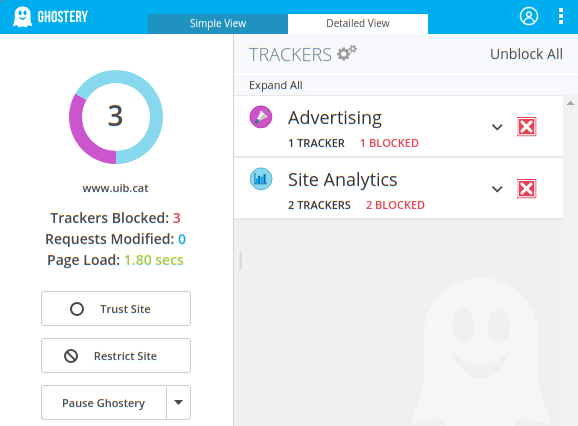
\includegraphics[scale=0.6]{ghost_uib.png}\\
  \caption{Trackers de UIB}
  \label{fig:object}
\end{figure}

\begin{figure}[H]
  \centering
  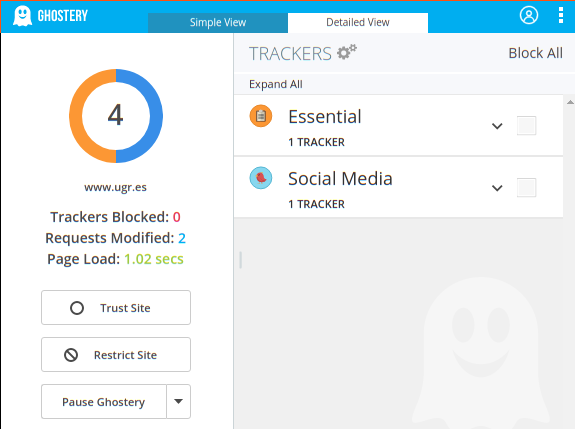
\includegraphics[scale=0.6]{ghost_ugr.png}\\
  \caption{Trackers de UGR}
  \label{fig:object}
\end{figure}

\begin{figure}[H]
  \centering
  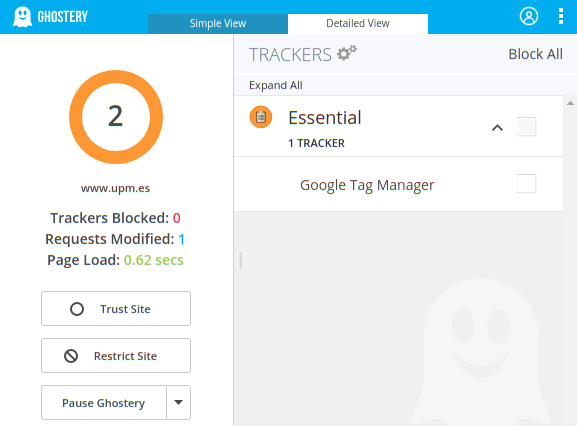
\includegraphics[scale=0.6]{ghost_upm.png}\\
  \caption{Trackers de UPM}
  \label{fig:object}
\end{figure}


\subsubsection*{Redes sociales}

\begin{figure}[H]
  \centering
  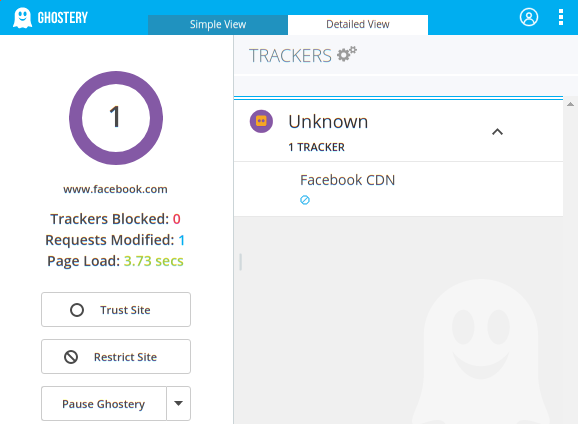
\includegraphics[scale=0.6]{ghost_fb.png}\\
  \caption{Trackers de Facebook}
  \label{fig:object}
\end{figure}

\begin{figure}[H]
  \centering
  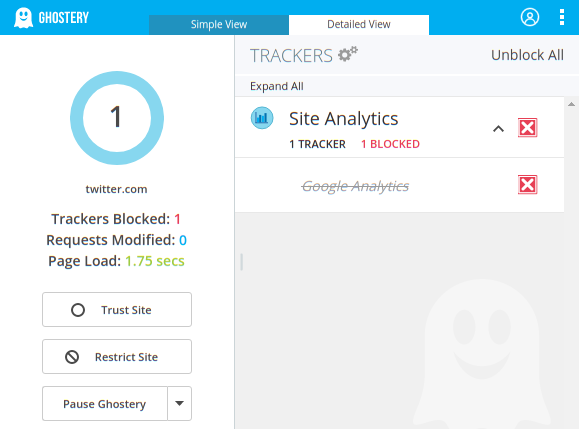
\includegraphics[scale=0.6]{ghost_twitter.png}\\
  \caption{Trackers de Twitter}
  \label{fig:object}
\end{figure}

\begin{figure}[H]
  \centering
  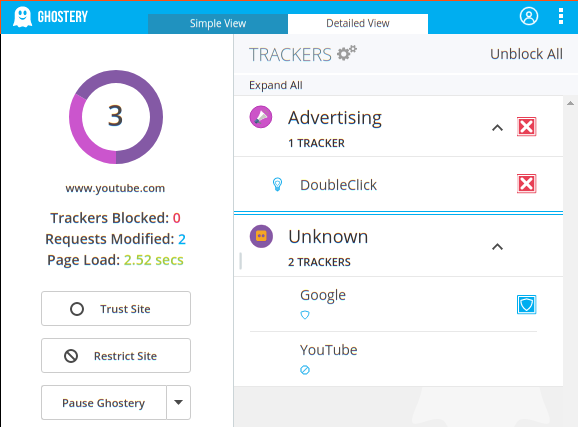
\includegraphics[scale=0.6]{ghost_youtube.png}\\
  \caption{Trackers de YouTube}
  \label{fig:object}
\end{figure}

\subsubsection*{Tiendas online}

\begin{figure}[H]
  \centering
  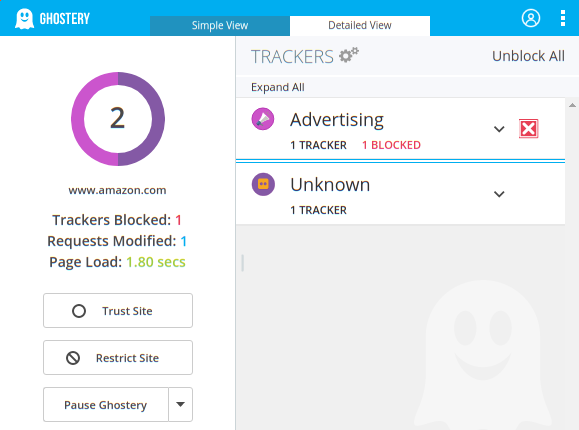
\includegraphics[scale=0.6]{ghost_amazon.png}\\
  \caption{Trackers de Amazon}
  \label{fig:object}
\end{figure}

\begin{figure}[H]
  \centering
  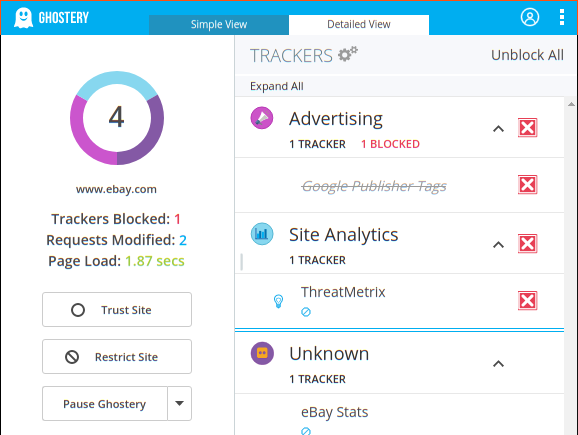
\includegraphics[scale=0.6]{ghost_ebay.png}\\
  \caption{Trackers de eBay}
  \label{fig:object}
\end{figure}

\begin{figure}[H]
  \centering
  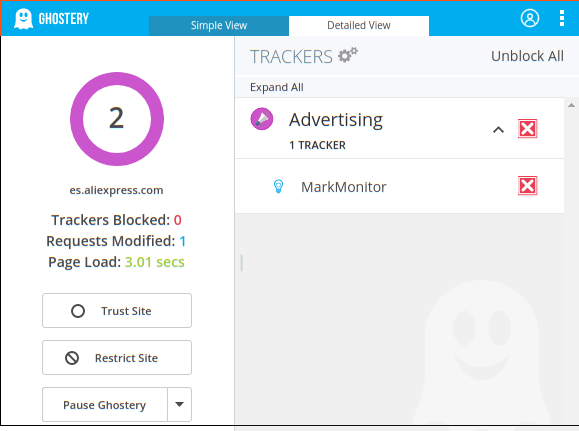
\includegraphics[scale=0.6]{ghost_aliexpress.png}\\
  \caption{Trackers de Ali Express}
  \label{fig:object}
\end{figure}

\subsubsection*{Resultados}

	\hskip-3.5cm
    \begin{tabular}{| c | c | c | c | c | c | c | c |}
    \hline
     	& Advertising & Essential & Site Analytics & Social Media & Customer Interaction & Unknown & Total\\ \hline
    El País & 5 & - &  3 & 1 & - & 1 & 10 \\ \hline
    El Mundo & 8 & 1 & 4 & - & 1 & 1 & 15 \\ \hline
    20 minutos & 2 & 1 & 1 & - & - & 1 & 5 \\ \hline
    Última Hora & 1 & 1 & 2 & - & - & 1 & 5 \\ \hline
    La Razón & 1 & 1 & 1 & - & - & 1 & 4 \\ \hline
    La Sexta & 3 & 1 & 5 & - & - & 1 & 10 \\ \hline
    UOC & 1 & 1 & 2 & - & - & 2 & 6 \\ \hline
    URV & - & 1 & - & - & - & - & 1 \\ \hline
    UAB & - & 1 & - & - & - & - & 1 \\ \hline
    UIB & 1 & - & 2 & - & - & 1 & 4 \\ \hline
    UGR & - & 1 & - & 1 & - & - & 2 \\ \hline
    UPM & - & 1 & - & - & - & - & 1 \\ \hline
    Facebook & - & - & - & - & - & 1 & 1 \\ \hline
    Twitter & - & - & 1 & - & - & - & 1  \\ \hline
    YouTube & 1 & - & - & - & - & 2 & 3 \\ \hline
    Amazon & 1 & - & 1 & - & - & 1 & 3  \\ \hline
    eBay & 1 & - & 1 & - & - & 1 & 3 \\ \hline
    Ali Express & 1 & - & - & - & - & - & 1 \\ 
    \hline
    \end{tabular}
    \begin{center}
	Recuento de trackers en páginas web
    \end{center}
    
    \begin{center}
		\begin{tabular}{| c | c |}
	    \hline
     		& Total \\ \hline
	    Advertising & 26 \\ \hline
    	Essential & 10 \\ \hline
	    Site Analytics & 23 \\ \hline
    	Social Media & 2 \\ \hline
    	Customer Interaction & 1 \\ \hline
    	Unknown & 14 \\
    	\hline
	    \end{tabular}    
    \end{center}
    
\vspace{1cm}

Las páginas web que incluyen mayor seguimiento con una amplia diferencia a las demás son las páginas de El Mundo, El País y La Sexta, las 3 son páginas de medios de comunicación.\\

Los seguimientos más frecuentes en todas las páginas son los de Advertising, especialmente en las de tipo de medio de comunicación. Para páginas del tipo Universidades también hay Advertising y se destacan los trackers de Site Analytics. Las redes sociales cuentan con muy pocos trackers, se destacan los de tipo desconocido. Por otra parte, las páginas de tiendas online también hay más trackers de tipo Advertising en comparación a las demás.\\

En cuanto a los resultados, no me ha sorprendido ver que la mayoría de trackers son del tipo Advertising y Site Analytics, sin embargo, me sorprende ver que las páginas de medios de comunicación son las que más trackers poseen en comparación a las redes sociales o tiendas online.

\section{}
\subsection{}
El fingerprinting a través del explorador consiste en construir un perfil a través de la información de configuración y otros datos que se pueden obtener de un explorador que navega por internet. Debido a la cantidad y naturaleza específica de los datos del explorador se puede construir lo que sería una huella digital del explorador y, por tanto, del usuario que lo esté usando. Al contrario de las cookies, esta construcción consiste en un proceso pasivo, pues no se tiene que depositar ningún tipo de información en el cliente de la sesión.\\

Repercute en varios ámbitos de la privacidad del usuario ya que este proceso no es algo que el usuario pueda escoger participar de él (al contrario que con las cookies), depende completamente de sus conocimientos y habilidades el protegerse de estas medidas. Con la huella digital se puede obtener información muy valiosa porque a través de estos perfiles se puede llegar a distinguir a un usuario u a otro y, a su vez, utilizar esta información de la misma forma que una cookie convencional (publicidad a medida, patrones de uso, etc.).
\subsection{}
\begin{figure}[H]
  \centering
  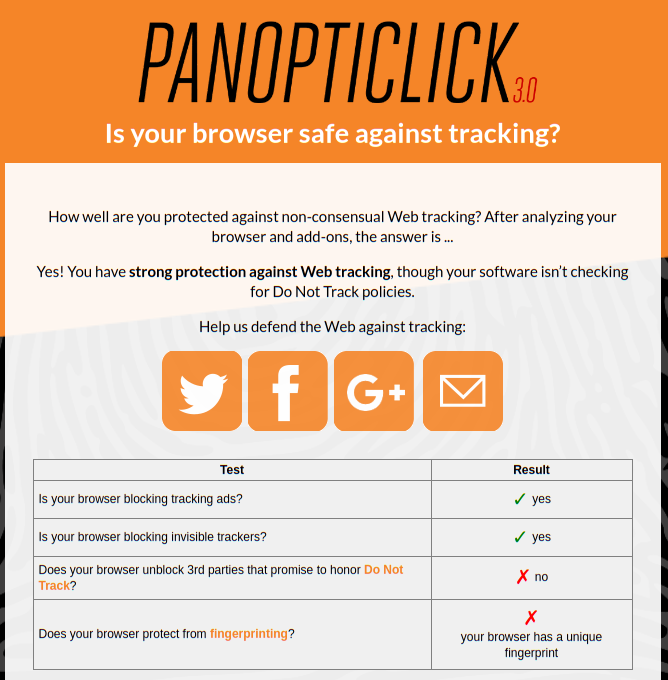
\includegraphics[scale=0.4]{p_chrome.png}\\
  \caption{Huella de Chrome}
  \label{fig:object}
\end{figure}

\begin{figure}[H]
  \centering
  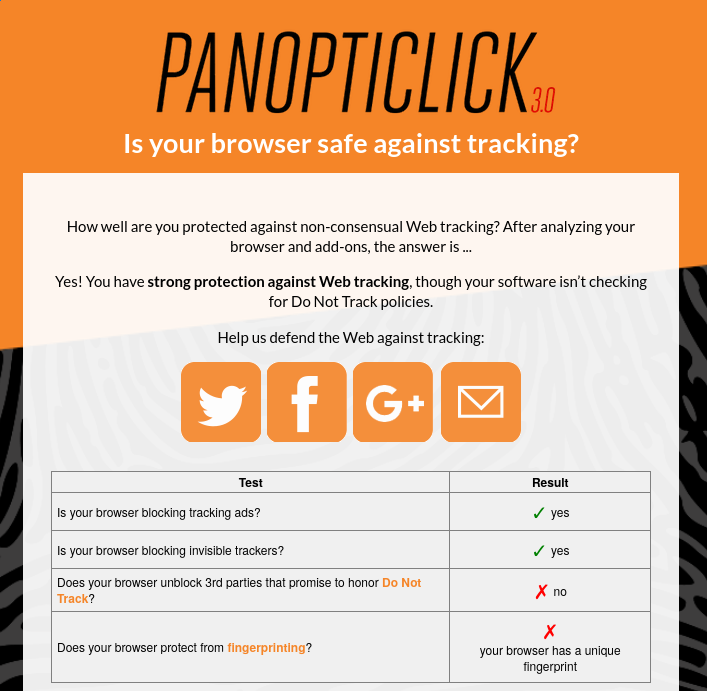
\includegraphics[scale=0.4]{p_firefox.png}\\
  \caption{Huella de Firefox}
  \label{fig:object}
\end{figure}

\begin{figure}[H]
  \centering
  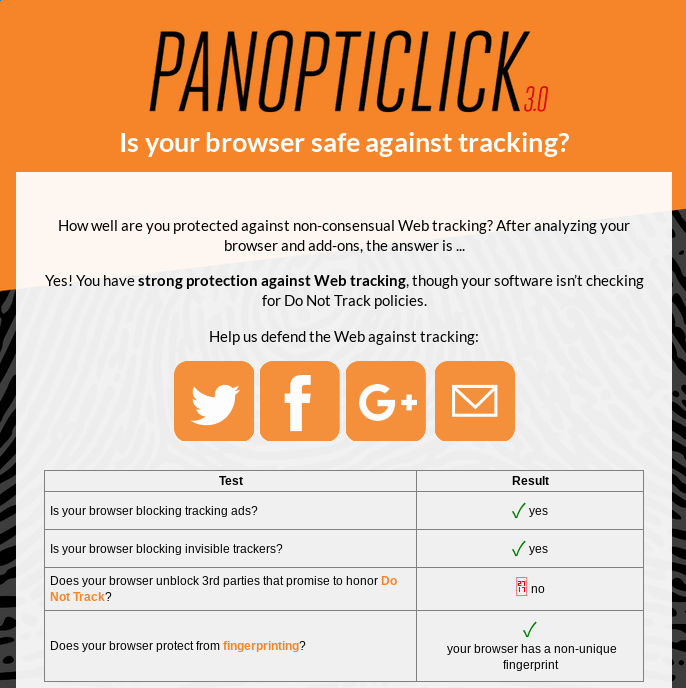
\includegraphics[scale=0.4]{p_tor.png}\\
  \caption{Huella de TOR}
  \label{fig:object}
\end{figure}

    \vspace{1cm}
    \begin{center}
		\begin{tabular}{| c | c | c | c |}
	    \hline
     		& Chrome & Firefox & TOR\\ \hline
	    Bloquea Tracking Ads & Sí & Sí & Sí \\ \hline
    	Bloquea Trackers invisibles & Sí & Sí & Sí \\ \hline
	    Bloquea Trackers de terceros dicen no traquear & No & No & No \\ \hline
    	Protege del fingerprinting & No & No & Sí \\
    	\hline
	    \end{tabular}    
    \end{center}

Tanto Chrome como Firefox dan los mismo resultados: Bloquean tracking ads y trackers invisibles. El único que protge del fingerprinting es TOR y ninguno de los 3 bloquea trackers de terceros que prometen no trackear.
\subsection{}
A continuación expongo las medidas que creo que son las más eficaces para combatir el fingerprinting a raíz de la lectura de estos artículos:\\

\subsubsection*{Plugins, extensiones y add-ons}
Los exploradores permiten añadir ciertos plugins que modifican la experiencia de navegación del usuario. Estos plugins permiten bloquear trackers y otro software que construye la huella digital del explorador.\\

\begin{itemize}
\item \textbf{Facilidad de uso}: Elevada, la mayoría de exploradores tienen algo similar a una store que permite buscar, instalar y configurar estos Add Ons
\item \textbf{Eficacia}: Dependiendo del plugin y de cómo se utilicen pueden ser efectivos o hasta contraproducentes porque añade parámetros de configuración que sean únicos al explorador.
\end{itemize}

\subsubsection*{Configuración del explorador. Modo de incógnito}
La mayoría de exploradores convencionales ofrecen al usuario la navegación en modo de incógnito, este modo hace al explorador obtener un perfil similar al de otros exploradores, haciendo la construcción de la huella digital aún más difícil. Además, este modo no acepta las cookies por defecto y otro software de tracking.\\

Los usuarios avanzados también pueden optar por entrar en la configuración del explorador y modificarlo al gusto para reducir su huella digital. Algunos exploradores como Firefox ofrecen opciones directamente relacionadas con el fingerprinting e incluso cargar perfiles hechos a medida por sus usuarios.

\begin{itemize}
\item \textbf{Facilidad de uso}: Media-baja. Utilizar el modo incógnito es una opción ampliamente conocida por el usuario medio de internet. La configuración personal quizá ya requiere de conocimientos avanzados y queda bajo la responsabilidad del usuario.
\item \textbf{Eficacia}: Utilizar el modo incógnito reduce considerablemente las posibilidades de tener una huella única. En cuanto a la eficacia de la opción de utilizar una configuración personalizada dependerá del nivel de conocimientos del usuario.
\end{itemize}

\subsubsection*{TOR y VPN}
Esta creo que es la medida más eficaz. Consiste en utilizar TOR sobre una VPN de tal forma que conseguimos utilizar un explorador con alto grado de anonimidad sobre una red que nos permite navegar de manera anónima y sin tener que utilizar los relays de TOR, teniendo así la experiencia de TOR pero con la velocidad que ofrece una VPN.\\

\begin{itemize}
\item \textbf{Facilidad de uso}: Muy baja, esta solución requiere de una VPN que es una solución de pago y configurar TOR. Requiere de conocimientos avanzados para su configuración y uso.\\
\item Eficacia: En mi opinión es la más eficaz. Ofrece anonimidad por ambas partes, tanto desde el punto de vista de la red como el de explorador haciendo así la huella digital aún más difícil de perfilar.
\end{itemize}

\subsection{}
La técnica del \textit{(Cross-)Browser fringerprinting} consiste en sacar la huella digital mediante el explorador realizando una serie de tareas que utilizan el estándard WebGL para renderizar 3D en los exploradores. Estas tareas se pueden realizar mediante JavaScript con un proceso paralelo mientras el usuario navega por la página y se recogen datos basados en el sistema operativo y el hardware del usuario. De esta forma, se puede crear una huella digital para un mismo usuario independientemente del número de exploradores que utilice.\\  

A diferencia del fingerprint tradicional, este nuevo método llega a capas inferiores del ordenador del usuario y obvia cualquier tipo de software que este utilice para navegar por internet. Su ventaja reside en que ahora el perfil del usuario puede ser construido e identificable independientemente de las medidas que utilice el usuario, exceptuando TOR o deshabilitando completamente JavaScript en las páginas donde navegue. Como desventaja tenemos que estas operaciones sobre WebGL quizá no sean compatible con todos los exploradores y no se pueda realizar el fingerprinting en versiones antiguas de los mismos.

\end{document}